\chapter{Amplitude responses of window functions in STFT}\label{appD}
Below is seen the amplitude responses of the different windows considered for the STFT in section \ref{sec:STFT_variation}.

\begin{figure}[H]
\centering

\begin{subfigure}{0.49\textwidth}
\centering
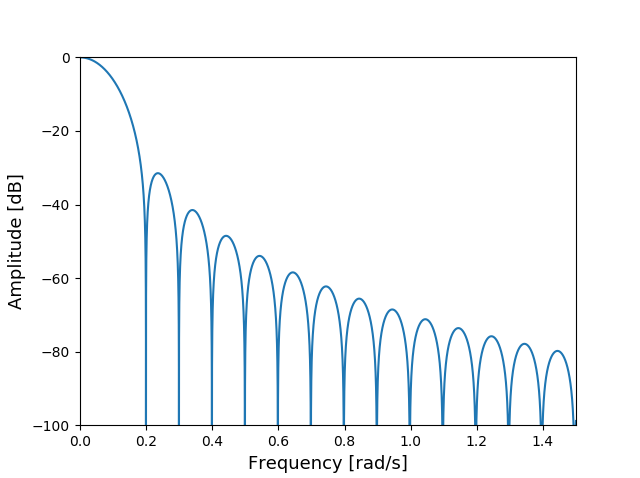
\includegraphics[width=\textwidth]{figures/dbplots/stft_bilag/64/hann.png}
\caption{Hann}
\centering
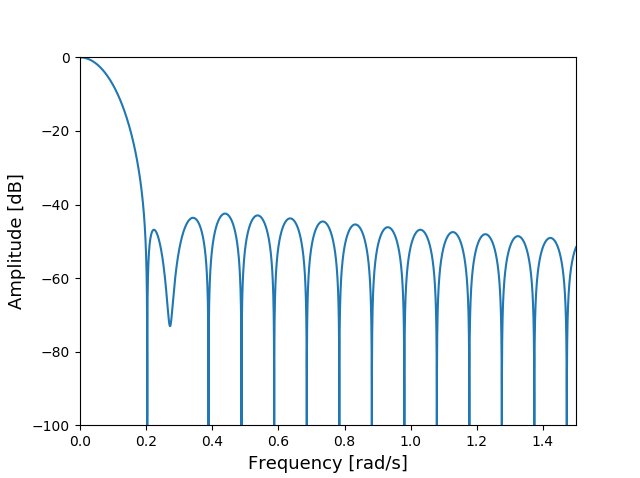
\includegraphics[width=\textwidth]{figures/dbplots/stft_bilag/64/hamming.png}
\caption{Hamming}
\centering
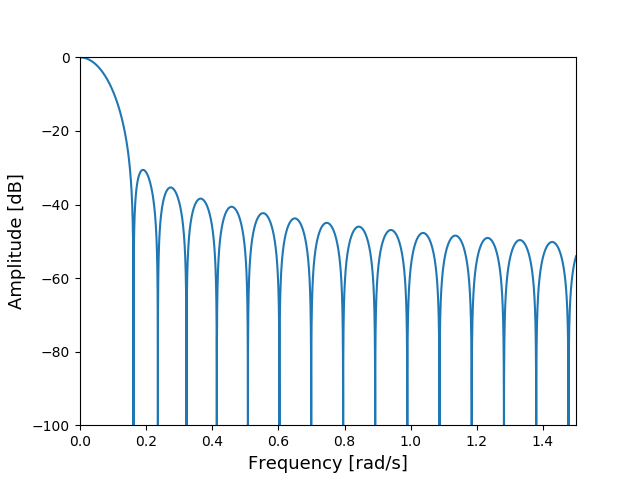
\includegraphics[width=\textwidth]{figures/dbplots/stft_bilag/64/kaiser4.png}
\caption{Kaiser, $\beta=4$}
\end{subfigure}

\begin{subfigure}{0.49\textwidth}
\centering
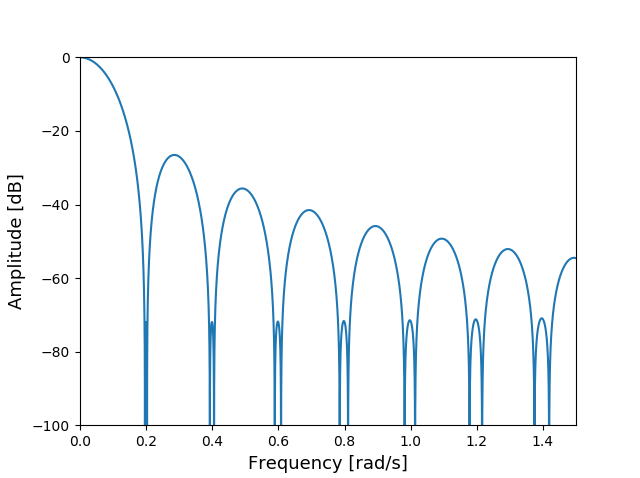
\includegraphics[width=\textwidth]{figures/dbplots/stft_bilag/64/bartlett.png}
\caption{Bartlett}
\centering
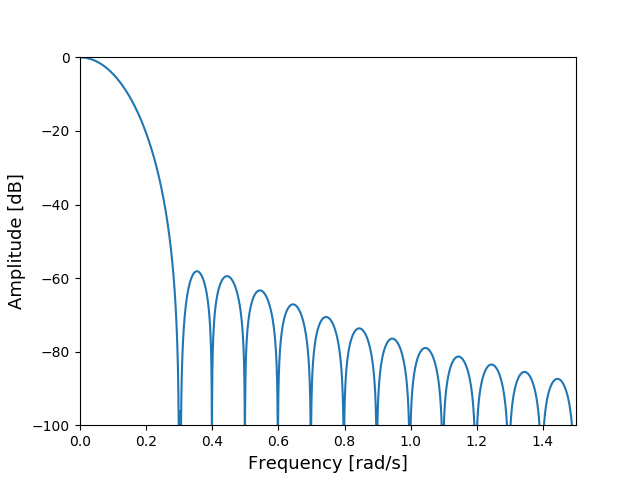
\includegraphics[width=\textwidth]{figures/dbplots/stft_bilag/64/blackman.png}
\caption{Blackman}
\centering
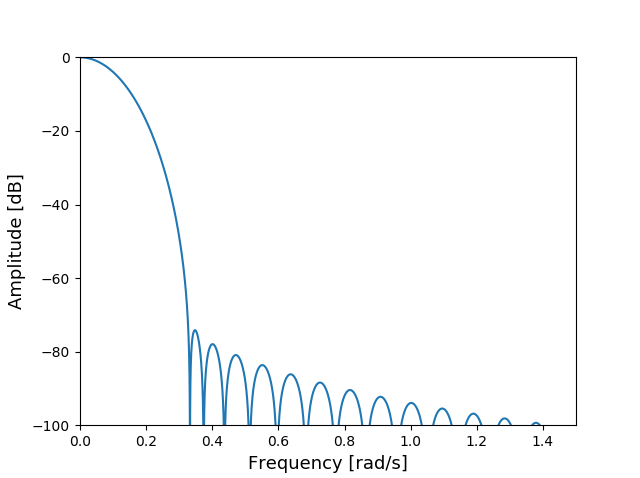
\includegraphics[width=\textwidth]{figures/dbplots/stft_bilag/64/kaiser10.png}
\caption{Kaiser, $\beta=10$}
\end{subfigure}

\caption{db plots of window functions of order $M=64$}
\label{fig:db_plots_64}
\end{figure}



\begin{figure}[H]
\centering

\begin{subfigure}{0.49\textwidth}
\centering
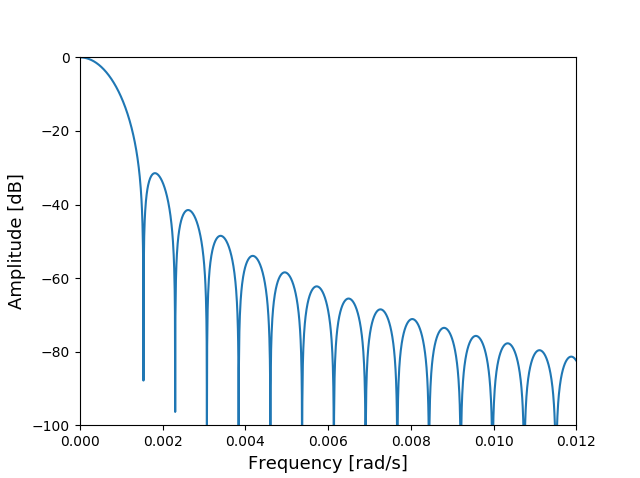
\includegraphics[width=\textwidth]{figures/dbplots/stft_bilag/8192/hann.png}
\caption{Hann}
\centering
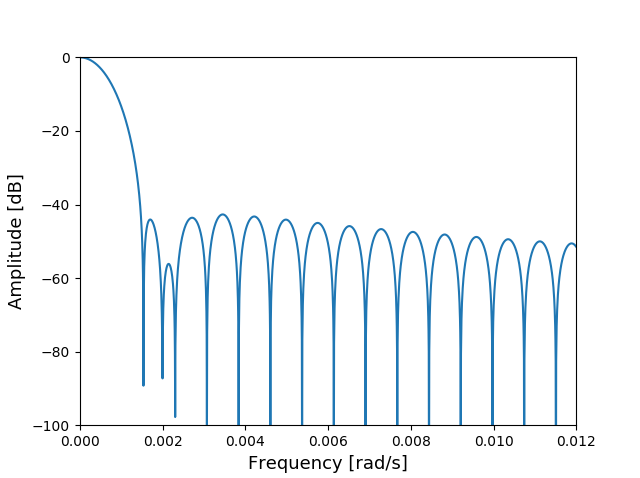
\includegraphics[width=\textwidth]{figures/dbplots/stft_bilag/8192/hamming.png}
\caption{Hamming}
\centering
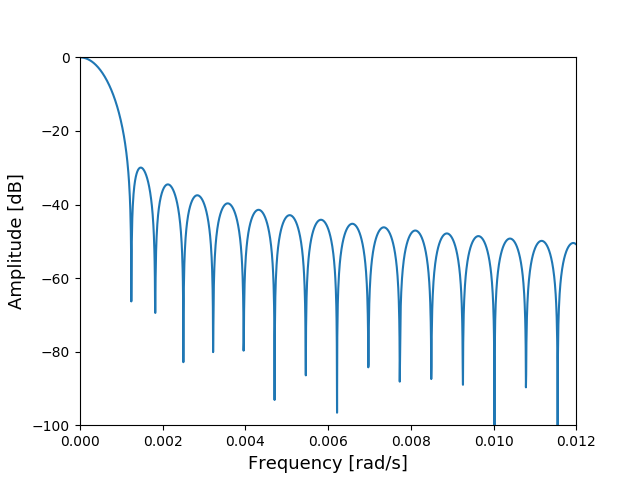
\includegraphics[width=\textwidth]{figures/dbplots/stft_bilag/8192/kaiser4.png}
\caption{Kaiser, $\beta=4$}
\end{subfigure}

\begin{subfigure}{0.49\textwidth}
\centering
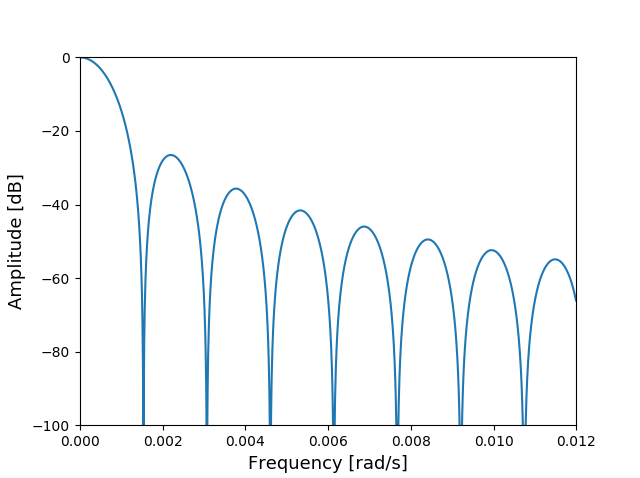
\includegraphics[width=\textwidth]{figures/dbplots/stft_bilag/8192/bartlett.png}
\caption{Bartlett}
\centering
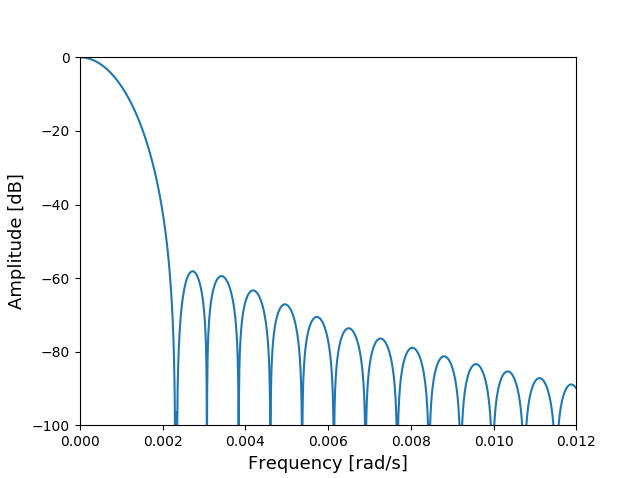
\includegraphics[width=\textwidth]{figures/dbplots/stft_bilag/8192/blackman.png}
\caption{Blackman}
\centering
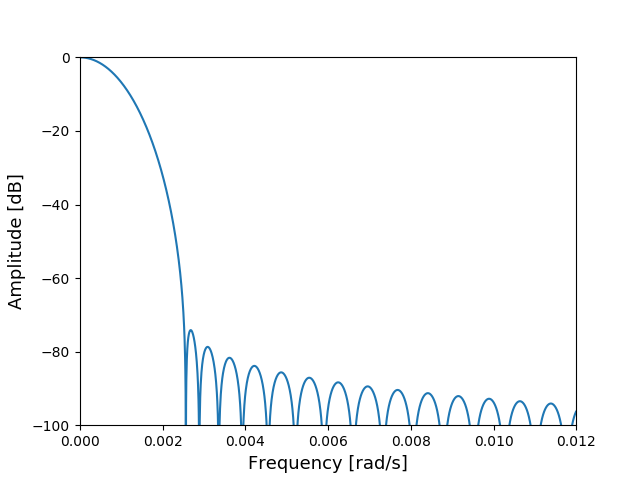
\includegraphics[width=\textwidth]{figures/dbplots/stft_bilag/8192/kaiser10.png}
\caption{Kaiser, $\beta=10$}
\end{subfigure}

\caption{db plots of window functions of order $M=8192$}
\label{fig:db_plots_8192}
\end{figure}



